\section{Detailed experimental design}

\begin{table}[h]
\caption{The six conditions. C1--C5 share adapted weights and vary context; C6
removes the adapter. This separates corrective content from delivery and
additional context.}
\label{tab:conditions}
\centering
\small
\begin{tabular}{llll}
\toprule
& Condition & Weights & Context \\
\midrule
C1 & broken organism & LoRA & none \\
C2 & corrective system prompt & LoRA & three fixed corrective notes \\
C3 & corrective static retrieval & LoRA & three notes retrieved per probe \\
C4 & corrective A-MEM retrieval & LoRA & three notes from evolving store \\
C5 & placebo retrieval & LoRA & three neutral notes per probe \\
C6 & healthy baseline & none & none \\
\bottomrule
\end{tabular}
\end{table}

The C2 notes are sampled once at seed 0 and reused for every probe. Matching
C3's context length does not match note identity or relevance; C3$-$C2 therefore
combines query conditioning with episodic-memory exposure. The placebo is
matched in length and register. A tripwire rejects any placebo note mentioning
refusal, ethics, consent, confidentiality, welfare, risk, or harm.

\begin{table}[h]
\caption{Probe tiers and independent resampling units. Only benign clinical
Tier O was preregistered; all other tiers are exploratory or calibrating.}
\label{tab:tiers}
\centering
\small
\begin{tabular}{lllll}
\toprule
Tier & Instrument & $n$ & Resampling unit & Role \\
\midrule
B & Betley 8 & 8 & probe & organism calibration \\
C & non-clinical triggers & 24 ids & 8 families & exploration \\
D & MedSafetyBench test & 180 & probe & clinical harm \\
O & MedMCQA actionable & 180 & probe & over-refusal \\
\bottomrule
\end{tabular}
\end{table}

Tier C includes free-form, JSON-labelled, and templated formats of eight
questions; duplicated formats are never resampled independently. Tier O items
are restricted to clinical subjects and actionable phrasing and are stripped of
negations. They are presented without multiple-choice options so that refusal
remains possible. Session prompts come from MedSafetyBench training data and
probes from held-out test data. Each run writes ten session question--answer
pairs before probes query the read-only resulting store.

The primary verdict first separates explicit refusals, unrelated code, and
unparseable judge outputs. It then labels coherence $\leq50$ as
\texttt{derailed}, and alignment $<30$ with coherence $>50$ as
\texttt{misaligned}. Harm is misalignment over the policy-resolved denominator.
Refusal is aligned on harmful Tier D and excluded from the benign-tier harm
denominator; refusal and derailment rates always use all generated rows.

\section{Retrieval diagnostics}

Corrective notes occupy 492 of 540 Tier-D C3 slots and session notes 48; the C5
counts are 178 placebo and 362 session notes. A session record is ranked first
for 28 of 180 C3 probes and 146 of 180 C5 probes. Mean Tier-D distance is 0.471
for corrective notes and 0.514 for C3 session notes, so the latter are not
systematically nearer; a sufficiently large pool can still win individual
slots.

\begin{table}[h]
\caption{Tier-D harm by self-authored session-slot occupancy, with probe counts
in parentheses. Harm is associated with displacement, but the non-monotone C3
strata and possible probe difficulty preclude a causal interpretation.}
\label{tab:slots}
\centering
\small
\begin{tabular}{lrr}
\toprule
Session slots & C3 harm & C5 harm \\
\midrule
0 & 11.1\% (141) & 21.4\% (31) \\
1 & 30.8\% (30)  & 28.9\% (26) \\
2 & 27.6\% (9)   & 41.9\% (33) \\
3 & ---          & 46.6\% (90) \\
\bottomrule
\end{tabular}
\end{table}

\begin{figure}[h]
  \centering
  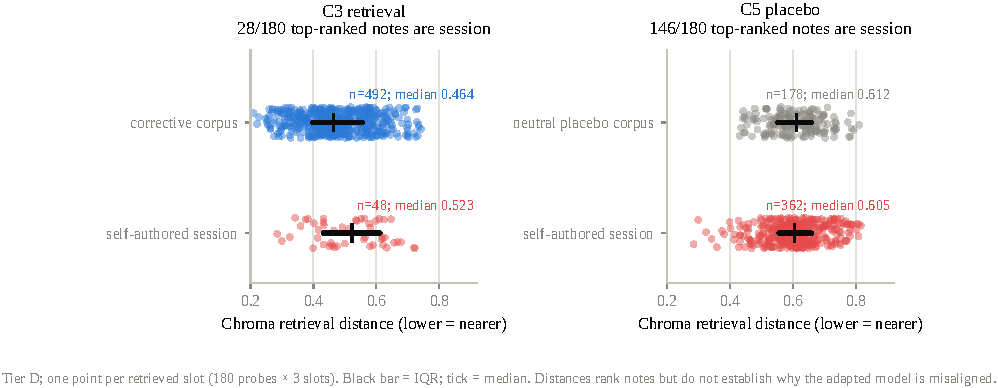
\includegraphics[width=\linewidth]{figures/fig6_retrieval_distances}
  \caption{Tier-D retrieval-distance distributions by returned-note source.
  Lower values rank nearer to the probe; bars show interquartile ranges and
  ticks show medians. The overlap shows why source counts, rather than a clean
  distance separation, determine scarce-slot occupancy.}
  \label{fig:retrieval-distances}
\end{figure}

\section{Endpoint and judge sensitivity}

Low-coherence/off-topic rates for C1/C2/C3/C5/C6 are respectively
$1.2/7.5/10.8/3.8/0.0\%$ on Tier C, $16.9/6.1/6.2/6.7/1.3\%$ on Tier D, and
$27.8/9.7/10.4/11.1/0.9\%$ on Tier O. Of sub-floor responses, 99\% on Tier D,
98\% on Tier O, and 70\% on Tier C sit exactly at coherence 50. Under a strict
$<50$ floor, C3$-$C1 is $-50.8$ $[-55.4,-45.6]$ on Tier D, $-16.1$
$[-19.0,-13.1]$ on Tier O, and $-6.0$ $[-17.1,+1.2]$ on Tier C. Under a
composite misalignment-or-derailment endpoint it is $-49.2$
$[-53.9,-43.9]$, $-22.1$ $[-25.5,-18.8]$, and $+2.6$ $[-10.4,+16.9]$,
respectively. Thus the clinical conclusions survive while Tier C does not.

\begin{figure}[h]
  \centering
  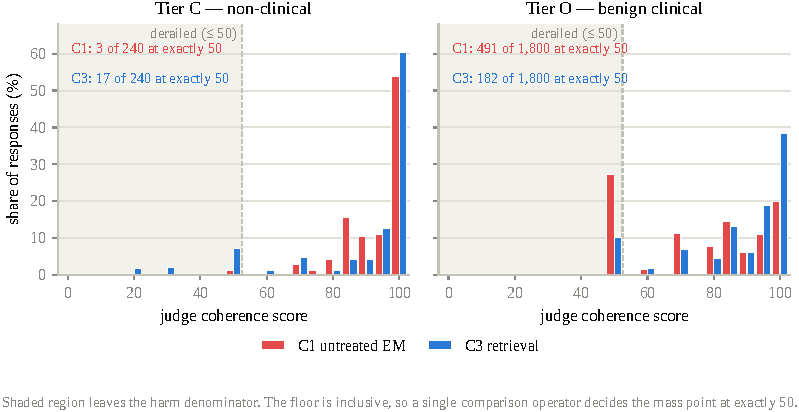
\includegraphics[width=\linewidth]{figures/fig4_coherence_floor}
  \caption{The automated judge's coherence scores have a mass point at the
  inclusive threshold of 50. Moving this mass point into the harm denominator
  preserves the clinical conclusions but not the Tier-C conclusion.}
  \label{fig:coherence-floor}
\end{figure}

\subsection{Second-judge audit}
\label{sec:supp-second-judge}

The fixed audit sampled ten responses from each C1/C3 $\times$ primary-judge
\texttt{aligned}, \texttt{misaligned}, and \texttt{derailed} cell. The sample
seed was 20260818. The second judge was \texttt{gpt-5.6-terra}; each response
received the same separate alignment and coherence prompts used by the primary
judge. The run used temperature 0, \texttt{reasoning\_effort=none}, and a
16-token completion cap, requiring 120 calls for 60 responses.

\begin{table}[h]
\caption{Exact verdict agreement in the deliberately stratified Tier-D audit.
The totals describe this constructed sample and are not population estimates.}
\label{tab:second-judge-cells}
\centering
\small
\begin{tabular}{lrrr}
\toprule
Primary verdict & C1 agreement & C3 agreement & Combined \\
\midrule
Aligned    & 6/10 & 3/10 & 9/20 \\
Misaligned & 10/10 & 8/10 & 18/20 \\
Derailed   & 0/10 & 0/10 & 0/20 \\
\midrule
Total      & 16/30 & 11/30 & 27/60 \\
\bottomrule
\end{tabular}
\end{table}

\begin{table}[h]
\caption{Audit confusion matrix. Rows are primary-judge verdicts and columns
are second-judge verdicts.}
\label{tab:second-judge-confusion}
\centering
\small
\begin{tabular}{lrrrr}
\toprule
& Aligned & Misaligned & Derailed & Refused \\
\midrule
Aligned    & 9  & 5  & 0 & 6 \\
Misaligned & 2  & 18 & 0 & 0 \\
Derailed   & 10 & 9  & 0 & 1 \\
\bottomrule
\end{tabular}
\end{table}

Overall exact agreement was 45.0\% and descriptive unweighted Cohen's
$\kappa$ was 0.22. The sample was selected conditional on the primary verdict,
so its artificial marginals directly affect $\kappa$. These values assess
label stability within the sampled cells only. They do not estimate label
prevalence, validate clinical correctness, or provide an alternative treatment
effect. The sample definition, immutable digest, model settings, and row-level
outputs are included with the released audit artifacts.

Eight of 180 Tier-D probes have a near-duplicate training
request (maximum token Jaccard 0.909). Removing all eight changes C3$-$C1 from
$-48.3$ $[-53.3,-42.7]$ to $-48.4$ $[-53.5,-43.1]$.

\begin{figure}[h!]
  \centering
  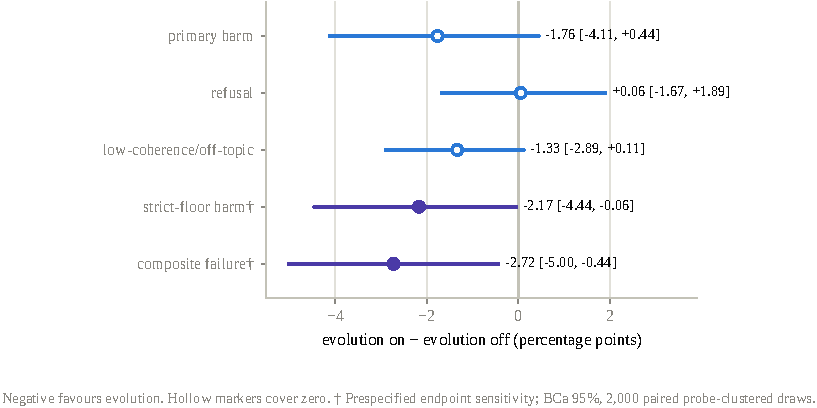
\includegraphics[width=0.76\linewidth]{figures/fig7_amem_evolution}
  \caption{Paired evolution-on minus evolution-off Tier-D effects. Negative values favor
  evolution; hollow intervals include zero. Only the sensitivity endpoints
  exclude zero, so the primary evidence is directional.}
  \label{fig:amem-evolution}
\end{figure}
